\section{Silná a slabá formulace 1D okrajové úlohy 2. řádu}

Řešme jednoduchou úlohu vedení tepla. 

Představme si zjednodušeně termosku jako 1D úsečku (oblast $\Omega = [0,1]$),
která na jedné straně (na dně) nepropouští žádné teplo a na straně druhé je otevřená,
tedy v kontaktu s okolím o referenční teplotě 0 (řekněme, že tu můžeme libovolně škálovat, např. že odpovídá 25$^\circ$C).

Zaveďme si veličinu $q(x,t)$, která bude popisovat hustotu energie (tepla) uvnitř oblasti $\Omega$.
Oblast $\Omega$ je interval, jedná se tedy v tomto případě o délkovou hustotu.
Může se samozřejmě měnit v čase $t$.
Celkovou energii v oblasti $\Omega$ v čase $t$ tedy vyjádříme jako
\[
  \int\limits_0^1 q(x,t) \d x
\]
Dále si zaveďme tepelný tok $j(x,t)$, který vyjadřuje kolik energie projde bodem $x$ (představujeme si příčný průrez termoskou)
za jednotku času.
Nyní můžeme vyjádřit úbytek energie jako zápornou změnu celkové energie v čase a tu položit rovnu rozdílu tepelného toku
na začátku a konci oblasti, tedy v bodech $x=0$ a $x=1$.
\[
  -\frac{\partial}{\partial t}\int\limits_0^1 q \d x = j(1) - j(0) = \int\limits_0^1 \frac{\partial j}{\partial x} \d x
\]
Dostali jsme energetickou bilační rovnici. Pokud budeme předpokládat, že $j$ je hladkou funkcí podle $x$, můžeme rozdíl tepelných toků nahradit 
integrálem derivace $j$ přes danou oblast.

Dále si můžeme představit, že stěny termosky přece jen nejsou ideální a i přes ně probíhá výměna tepla.
Tedy zavedeme funkci $f(x)$, která bude popisovat dodávání ($f(x)>0$) nebo odebírání ($f(x)<0$) energie z venku do/z oblasti $\Omega$.
Tím získáme následující bilanční rovnici:
\[
  -\frac{\partial}{\partial t}\int\limits_0^1 q \d x = j(1) - j(0) + \int\limits_0^1 f(x) \d x= \int\limits_0^1 \left(\frac{\partial j}{\partial x} + f(x) \right) \d x
\]

....

\[
  \frac{\partial q}{\partial t} + \frac{\partial j}{\partial x} = f(x)
\]
Pokud budeme uvažovat ustálenou úlohu, tedy časově neměnnou, zjednoduší se rovnice na
\begin{equation}
  j'(x) = f(x) \label{eqn:continuity_steady_1d}
\end{equation}

Nyní připomeňme Fourierův zákon, který definuje tepelný tok pomocí gradientu teploty
\begin{equation}
j(x) = -K(x)u'(x), \label{eqn:fourier_1d}
\end{equation}
kde $K(x)$ je tepelná vodivost materiálu.


Pokud nyní dosadíme \eqref{eqn:fourier_1d} do \eqref{eqn:continuity_steady_1d}, dostaneme Poissonovu rovnici,
a poté popíšeme náš problém termosky
% \[
% -(K(x)u'(x))' = f(x)
% \]

\begin{eqnarray}
-(Ku')'(x) &=& f(x) \qquad \textrm{in } \Omega = [0,1], \label{eqn:poisson}\\
-(Ku')(0) &=& 0, \label{eqn:hom_neumann}\\
u(1) &=& 0, \label{eqn:hom_dirichlet}
\end{eqnarray}
kde \eqref{eqn:poisson} řídí rozložení teploty $u(x)$ uvnitř termosky,
\eqref{eqn:hom_neumann} je homogenní Neumannovou okrajovou podmínkou a vyjadřuje nulový tepelný tok skrz dno termosky
a \eqref{eqn:hom_dirichlet} je homogenní Dirichletovou okrajovou podmínkou a pokládá teplotu na otevřeném konci termosky rovnou nule.


Slabou formulaci získáme přenásobením \eqref{eqn:poisson} testovací funkcí $\varphi(x)\in\mathcal{C}([0,1])$, $\varphi(1)=0$, 
následnou integrací rovnice přes oblast $\Omega$ a aplicaí okrajových podmínek za použití per partes (resp. Greenovy věty).
\[
  \int\limits_{\Omega} -\left( Ku'\right)'(x) \varphi(x) \d x = \int\limits_{\Omega} f(x) \varphi(x) \d x
\]

\begin{equation}
\left[-\left( Ku'\right)(x)\varphi(x)\right]_0^1 + \int\limits_0^1 \left( Ku'\right)'(x) \varphi'(x) \d x
    = \int\limits_0^1 f(x) \varphi(x) \d x\label{eqn:weak_form}
\end{equation}
První člen daný okrajovými podmínkami je v našem případě nulový, díky Neumannově okrajové podmínce a volbě $\varphi$.

Integrální rovnici \eqref{eqn:weak_form} nazýváme slabou formulací problému \eqref{eqn:poisson}-\eqref{eqn:hom_dirichlet}.
Všimněme si dvou vlastností této formulace:
\begin{itemize}
  \item $u''$ nemusí existovat
  \item $u'$ nemusí být spojitá, stačí existence integrálu $\int_0^1(u')^2 \d x$
\end{itemize}

Označme nyní prostor, ze kterého pochází funkce $\varphi$:
\begin{equation}
  V = \{v\in H^1(\Omega); v(0) = 0\},
\end{equation}
kde prostor $H^1(\Omega)$ zaručuje pro funkce $\varphi$ výše zmíněnou druhou vlastnost,
a kde dále vidíme závislost $V$ na Dirichletově okrajové podmínce.
Z tohoto prostoru bude pocházet i řešení $u\in V$.

\paragraph{Galerkinova aproximace}
Nyní zvolíme konečně rozměrný vektorový podprostor $V_h\subset V$.
V tomto prostoru definujeme bázi $\{\varphi_j(x)\}_{j=1}^N$.
Tedy pro každou funkci $v_h\in V_h$ existuje právě jeden vektor $v_h^j,\, j=1\ldots N$,
takový že 
\[
  v_h(x) = \sum\limits_{j=1}^N v_h^j \varphi_j
\]

Uvažujme nyní aproximativní řešení $u_h\in V_h$ ve tvaru
\[
  u_h(x) = \sum\limits_{j=1}^N u^j_h \varphi_j
\]

Hledáme tedy $\vc u_h$ (vektor  koeficientů lineární kombinace), splňující \eqref{eqn:weak_form}
\[
  \int\limits_{\Omega} K(x) \left( \sum\limits_{j=1}^N u^j_h \varphi_j(x) \right)' \varphi_i'(x) \d x
    = \int\limits_{\Omega} f(x) \varphi_i(x) \d x \qquad \forall i=1\ldots N \label{eqn:discrete_weak_form}
\]
\begin{equation}
\sum\limits_{j=1}^N \underbrace{ \int\limits_{\Omega} K(x) \varphi'_j(x) \varphi_i'(x) \d x }_{A_{ij}} u^j_h
    = \underbrace{ \int\limits_{\Omega} f(x) \varphi_i(x) \d x }_{b_i} \qquad \forall i=1\ldots N \label{eqn:discrete_weak_form}
\end{equation}
čímž získáváme soustavu lineární algebraických rovnic
\begin{equation}
  \vc A \vc u_h = \vc b\label{eqn:linear_system}
\end{equation}

Uveďme si nyní dvě zásadní vlastnosti matice $\vc A$, a to symetrii
\begin{equation}
  A_{ij} = \int\limits_{\Omega} K(x) \varphi'_j(x) \varphi_i'(x) \d x = \int\limits_{\Omega} K(x) \varphi'_i(x) \varphi_j'(x) \d x = A_{ji}, \label{eqn:linear_system_symetry}
\end{equation}
a pozitivní definitnost
\begin{multline}
  \vc\alpha^T \vc A \vc\alpha = \sum\limits_{i,j=1}^N \alpha_i \alpha_j A_{ij}
  = \int\limits_{\Omega} K(x)
    \underbrace{\left( \sum\limits_{i=1}^N \alpha_i \varphi'_i(x) \right)}_{\vc v}
    \underbrace{\left( \sum\limits_{j=1}^N \alpha_j \varphi'_j(x) \right)}_{\vc v} \d x \\
  = \int\limits_{\Omega} K(x) |\vc v|^2 > 0 \quad \forall \vc v: |\vc v|\neq 0. \label{eqn:linear_system_pos_def}
\end{multline}
    
    
    
\subsection{Lineární konečné prvky v 1D}
Jako podprostor $V_h$ zvolíme množinu lineárních lomených funkcí na intervalu $[0,1]$.
Rozdělme interval $[0,1]$ pomocí bodů $x_0=0<x_1<x_2<...<x_{N}=1$ na intervaly $E_j:=(x_{j-1},x_j)$ o délce $h_j:=x_j-x_{j-1}$.
Normu tohoto dělení zavedeme jako $h:=\max_{j=1,...,N+1} h_j$.
Definujeme
\[ V_h:=\{v_h\in C([0,1]);~\forall j=1,...,N:~v_h \mbox{ je lineární na }E_j,~v_h(1)=0 \}. \]
%Jelikož funkce z $V_h$ jsou spojité a nulové v bodech $0$ a $1$, je automaticky $V_h$ podprostorem $H^1_0(0,1)$.
Každou funkci $v_h$ z $V_h$ jednoznačně určují její hodnoty v dělících bodech $\{x_j\}_{j=1}^N$.
Dimenze podprostoru tedy je $\dim V_h=N$.

Pro metodu konečných prvků je klíčová volba báze.
Zvolíme bázové funkce podprostoru $V_h$ pomocí vztahů
\begin{equation*}
      \varphi_i(x_j) = 
        \begin{cases}
          1 \quad \textrm{pro } i=j\\
          0 \quad \textrm{pro } i\neq j\\
        \end{cases}
\end{equation*}
Každá bázová funkce je tedy nenulová v právě jednom dělícím bodě (viz Obr. \ref{fig:base_1d_lin}).
\begin{figure}[h]
\centering
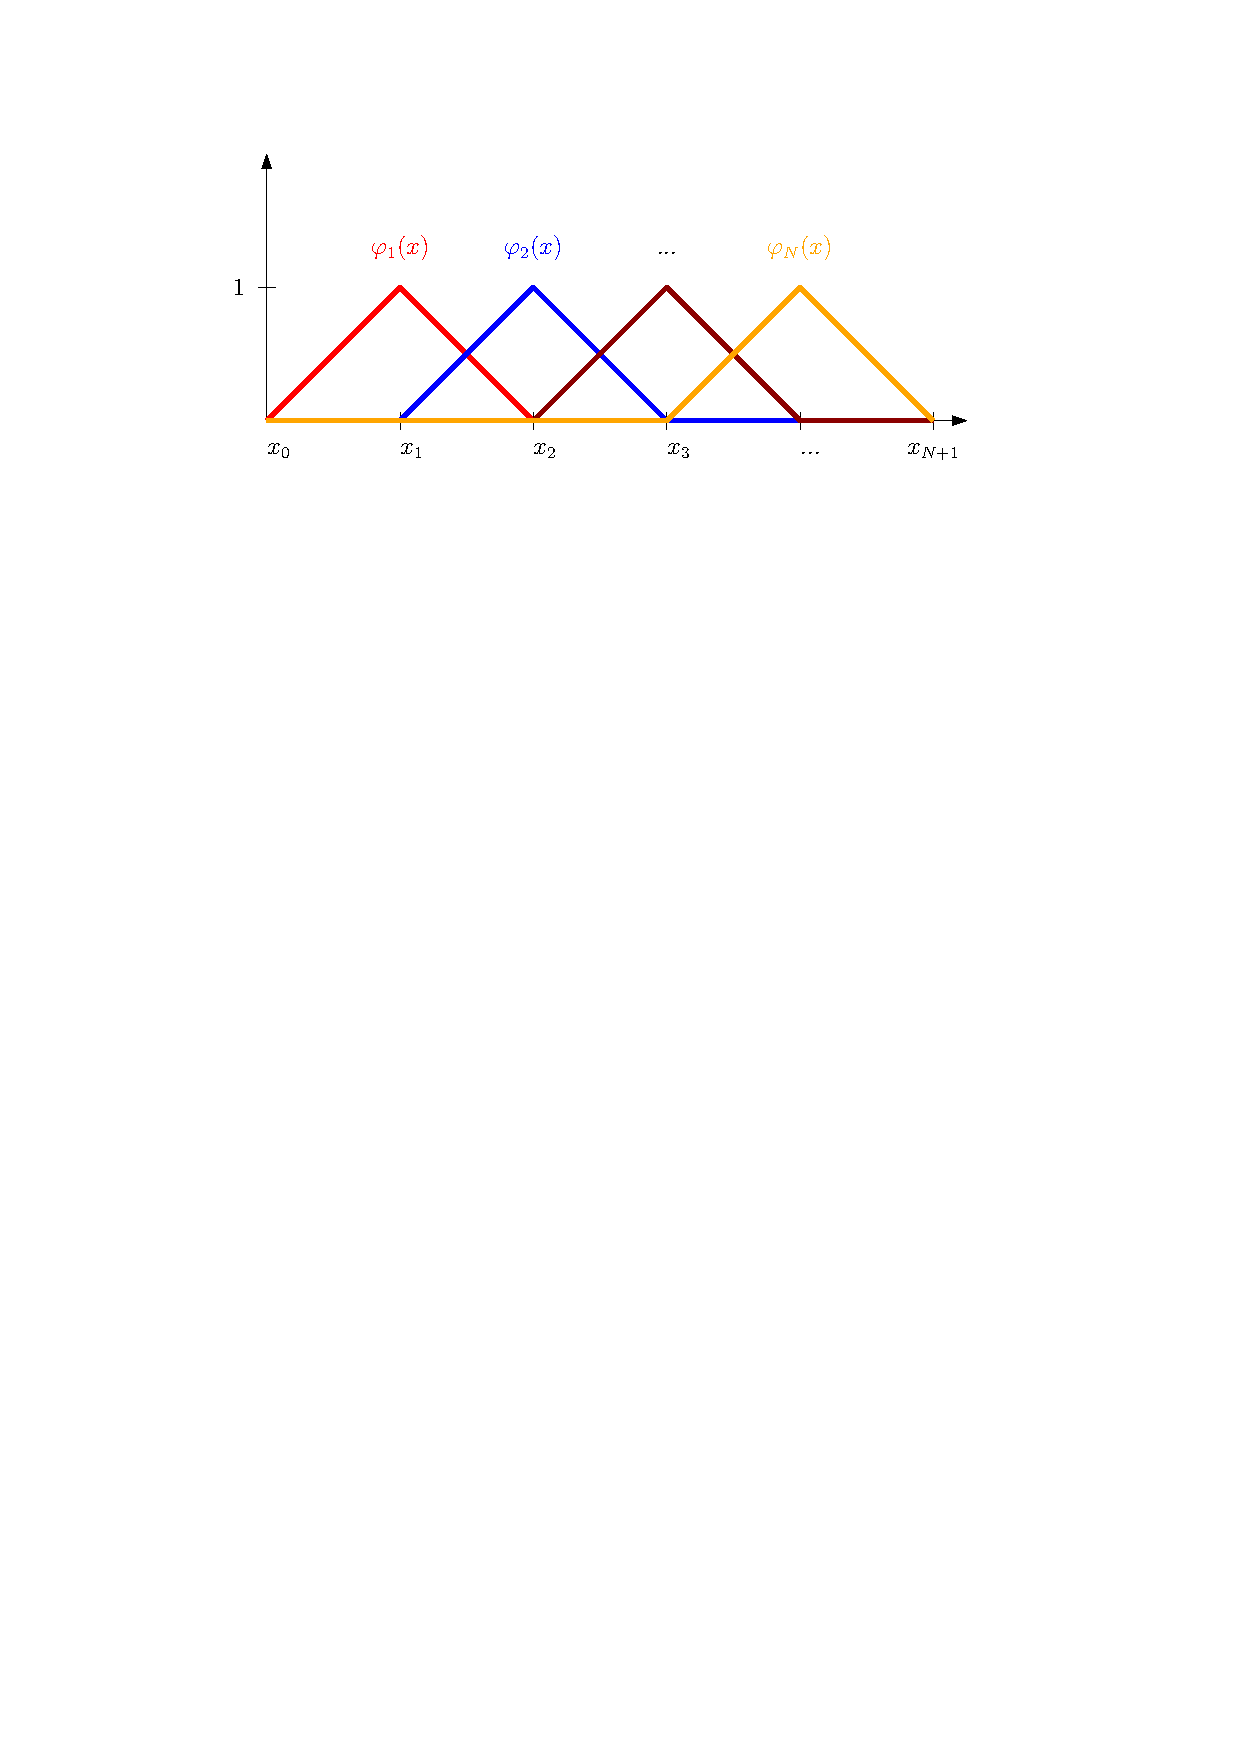
\includegraphics{base_1d_lin}
\caption{Bázové funkce pro prostor po částech lineárních funkcí.}
\label{fig:base_1d_lin}
\end{figure}
% Prvky matice $\tn A\in\R^{N\times N}$ a vektoru $\vc b\in\R^{N}$ mají tvar
% \[ a_{ij}=\int_0^1\varphi_j'(x)\varphi_i(x), \]
% \[ b_i = \int_0^1 f(x)\varphi_i(x)\d x. \]

Podívejme se nyní na konkrétní soustavu rovnic, kterou dostáváme.
Je zřejmé, že $A_{ij}$ je nulové, pokud se indexy $i$ a $j$ liší více než o 1, neboť v takovém případě je v každém bodě intervalu $(0,1)$ alespoň jedna z funkcí $\varphi_i$, $\varphi_j$ (a tedy i $\varphi_i'$, $\varphi_j'$) nulová. Matice $\vc A$ proto bude třídiagonální, a tedy řídká.

Pokud budeme uvažovat $K(x) = const.\, \forall x\in E_j,\, j = 1\ldots N$, pak platí:
\begin{align*}
A_{jj} &= \int_{x_{j-1}}^{x_j} K(x)\varphi_j'(x)^2\d x + \int_{x_j}^{x_{j+1}} K(x) \varphi_j'(x)^2\d x
= \int_{x_{j-1}}^{x_j}\frac{K}{h_{j-1}^2}\d x + \int_{x_j}^{x_{j+1}}\frac{K}{h_j^2}\d x\\
&= K\left(\frac1{h_{j-1}} + \frac1{h_j}\right),~j=1,...,N,\\\\
A_{j,j-1} &= A_{j-1,j} = \int_{x_{j-1}}^{x_j}K(x)\varphi_{j-1}'(x)\varphi_j'(x)\d x\\
&= \int_{x_{j-1}}^{x_j}\frac{(-K)}{h_{j-1}^2} \d x = -\frac{K}{h_{j-1}}, j=2,...,N.
\end{align*}
V případě ekvidistantního dělení ($h=h_j$ $\forall j=1,...,N$) a $K(x) = const.\, \forall x\in\Omega$ máme
\[ \tn A = \frac{K}{h}\begin{pmatrix}2 & -1 & \\-1 & 2 & -1\\\ddots&\ddots&\ddots\\&-1 & 2 & -1\\&& -1 & 2\end{pmatrix}. \]
% Protože bilineární forma $(a,u,v)$ je symetrická a eliptická, je také $\tn A$ symetrická a pozitivně definitní.
Soustava $\vc A\vc u_h=\vc b$ má řešení pro každý vektor $\vc b$,
%a řešením Galerkinovy úlohy je funkce $u_h(x):=\sum_{i=1}^N\xi_i\varphi_i(x)$.
hodnoty $u_h^i$ jsou zároveň hodnotami funkce $u_h$ v bodech $x_i$.

Podobně jako ve Větě \ref{th:cea} lze ukázat, že platí odhad chyby
\begin{equation}\label{eq:error_est_laplace_dir}
\forall v_h\in V_h:~\norm{u'-u_h'}_2 \le \norm{u'-v_h'}_2,
\end{equation}
takže $u_h$ je zároveň nejlepší aproximace slabého řešení $u$ v prostoru po částech lineárních funkcí.
Zvolme nyní vhodnou funkci $v_h$, abychom odhad chyby \eqref{eq:error_est_laplace_dir} vyjádřili kvantitativně.
Položíme $v_h:=\tilde u_h$, kde $\tilde u_h$ je interpolanta $u$ (po částech lineární funkce taková, že $\tilde u_h(x_i)=u(x_i)$, $i=0,...,N+1$).
Pak z teorie Lagrangeovy interpolace víme, že platí
\[ |u'(x)-\tilde u_h'(x)|\le h\max_{y\in[0,1]}|u''(y)| ~\forall x\in[0,1]. \]
Je-li funkce $u$ třídy $C^2([0,1])$, pak dostáváme odhad
\[ \norm{u'-u_h'}_2 \le \norm{u'-\tilde u_h'}_2 \le h\max_{y\in[0,1]}|u''(y)|, \]
který říká, že chyba Galerkinovy aproximace měřená jako $L^2$ norma rozdílu derivací je řádu $O(h)$.
